% Documentation.tex
%
\documentclass[11pt]{article}

%\usepackage{a4}     % DIN A4

%\usepackage[latin1]{inputenc}
%\usepackage[T1]{fontenc}

\usepackage[pdftex]{graphicx}
\usepackage{makeidx}
\makeindex


%\includeonly{definitions,base}
%\includeonly{definitions,bars}
%\includeonly{definitions,composite}
%\includeonly{definitions,direction}
%\includeonly{definitions,error}
%\includeonly{definitions,hbars}
%\includeonly{definitions,lines}
%\includeonly{definitions,linespoints}
%\includeonly{definitions,mountain}
%\includeonly{definitions,pareto}
%\includeonly{definitions,pie}
%\includeonly{definitions,points}
%\includeonly{definitions,split}
%\includeonly{definitions,stacked}

% Hyphenations
\hyphenation{init dataref}


\begin{document}

\pagenumbering{Roman} 
\title{Documentation of the Perl Package \textbf{Chart}}

%% Name der Autoren 
%% Die Adressenangaben werden mit \thanks{} eingeschlossen
%% Name des ersten Autors
\author{Chart Group\thanks{Bundesamt f�r Kartographie und Geod�sie, 
Geod�tisches Observatorium Wettzell, Sackenrieder Stra�e 25, 
D-93444 Bad K�tzting, E-mail: chart@fs.wettzell.de}}

\maketitle
\begin{center}
\Large Version 2.4.2
\end{center}

\clearpage
\texttt{\ttfamily}
\tableofcontents

% Einleitung
\pagenumbering{arabic}
%
% definitions.tex
% ---------------

% LENGTH
\newlength{\parabstand}
\setlength{\parabstand}{2ex plus1ex minus1ex}

\newlength{\itemabstand}
\setlength{\itemabstand}{1ex plus1ex minus1ex}

% Commands

\newcommand{\syn}[1]{
                      {\it\large #1}
                     } %Ende synopsis
\newcommand{\fett}[1]{
                       {\bf #1} 
                     }% Ende Hervorheben
\newcommand{\unl}[1] {
                      {\underline #1}
                     }%f�r implemet. und beschrei.
\newcommand{\kursiv}[1]{
                     {\it #1}
                     }
\newcommand{\herv}[1]{
                     {\underline{\bf\large #1}}
                     }

%-------------- command class -------------------------
\newcommand{\class}[1]{\textsc{\large #1}\index{Class!#1}}
%-------------- command module -------------------------
\newcommand{\module}[1]{\textsf{#1}}
%-------------- command parameter -------------------------
\newcommand{\parameter}[1]{\textit{#1}}

%-------------- command name -------------------------
\newcommand{\name}[1]{
   \parbox{15ex}{\underline{\bf\large Name:}} #1\index{#1}\\[\itemabstand]}

%-------------- command file -------------------------
\newcommand{\file}[1]{
   \parbox{15ex}{\underline{\bf\large File:}} #1\\[\itemabstand]}

%-------------- command requires -------------------------
\newcommand{\requires}[1]{
   \parbox{15ex}{\underline{\bf\large Requires:}} #1\\[\itemabstand]}
      
%-------------- command method -------------------------
\newcommand{\method}[1]{
      \parindent 0pt \textbf{#1}}
           
%-------------- command methodexplanation -------------------------
\newcommand{\methodexplanation}[1]{
      \hfill\parbox{0.9\textwidth}{\small\parindent 0pt #1}}


%-------------- command example -------------------------
\newcommand{\example}[1]{
      \parindent 0pt \mbox{\textbf{\footnotesize #1}}}   

%-------------- command Methods -------------------------
\newcommand{\Methods}
     {\parindent 0pt\underline{\bf\large Methods:}\\}
     
%-------------- command Attributes -------------------------
\newcommand{\Attributes}
     {\parindent 0pt\underline{\bf\large Attributes/Options:}\\}
     

%% Environment definitons
%  Environment Description
\newsavebox{\descriptionsavedbox}
\newenvironment{Description}
{\begin{lrbox}{\descriptionsavedbox}
 \begin{minipage}[t]{0.9\textwidth}
}%
{\vspace{\parabstand}
 \end{minipage}\end{lrbox}
 \parindent 0pt\underline{\bf\large Description:}
 \mbox{\usebox{\descriptionsavedbox}}
}% end Description


%  Environment Constructor
\newsavebox{\constructorsavedbox}
\newenvironment{Constructor}
{\begin{lrbox}{\constructorsavedbox}
 \begin{minipage}[t]{0.9\textwidth}
}%
{\vspace{\parabstand}
 \end{minipage}\end{lrbox}
 \parindent 0pt\underline{\bf\large Constructor:}
 \mbox{\usebox{\constructorsavedbox}}
}% end Constructor

%  Environment Example
\newsavebox{\examplesavedbox}
\newenvironment{Example}
{\begin{lrbox}{\examplesavedbox}
 \begin{minipage}[t]{0.9\textwidth}
}%
{\vspace{\parabstand}
 \end{minipage}\end{lrbox}
 \parindent 0pt{\large Example:}
 \mbox{\usebox{\examplesavedbox}}
}% end Example

% description.tex
%-----------------
\clearpage
\section{Description}
\synopsis

\begin{verbatim}
  use Chart::type;     (type is one of: Bars, Composite,
  Direction, ErrorBars, HorizontalBars, Lines, LinesPoints,
  Mountain, Pareto, Pie, Points, Split or StackedBars)

  $obj = Chart::type->new();
  $obj = Chart::type->new(\$width, \$height);

  $obj->set( $key_1,   $val_1, ... , $key_n,   $val_n);
  $obj->set( $key_1 => $val_1, ... , $key_n => $val_n);
  $obj->set( %hash );

  # GifGraph.pm-style API to produce PNG formatted charts:
  @data = ( \@x_tick_labels, \@dataset_1, ... , \@dataset_n);
  $obj->png( "filename", \@data );
  $obj->png( $filehandle, \@data );
  $obj->png( FILEHANDLE, \@data );
  $obj->cgi_png();

  # Graph.pm-style API:
  $obj->add_pt($label, $val_1, ..., $val_n);
  $obj->add_dataset($val_1, ..., $val_n);
  $obj->png("filename");
  $obj->png($filehandle);
  $obj->png(FILEHANDLE);
  $obj->cgi_png();
  # Similar functions are available for JPEG output.

  # Retrieve imagemap information:
  $obj->set('imagemap' => 'true');
  $imagemap_ref = $obj->imagemap_dump();

\end{verbatim}
\clearpage

The Perl module \class{Chart} creates \textsc{png} or \textsc{jpeg}
output which can be written to a file or to stdout. Therefore,
\class{Chart} can also create dynamic charts for web sites.

Many different chart types are available, viz., Bars,
Composite, Direction, ErrorBars, HorizontalBars, Lines, LinesPoints,
Mountain, Pareto, Pie, Points, Split, and StackedBars. Each
specific type is implemented as a class by itself which is
derived from the same abstract superclass, Base.

The hierarchy of \class{Chart} classes is shown in
Figure~\ref{fig:Aufbau}.

\begin{figure}[ht]
  \begin{center}
    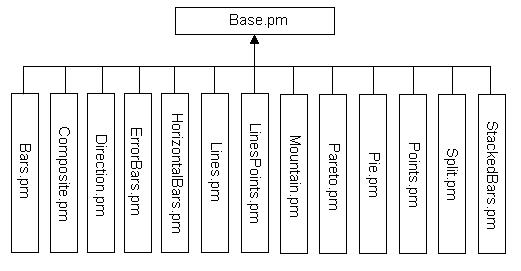
\includegraphics[scale=0.5]{Aufbau.png}
  \end{center}
  \caption{The hierarchy of \class{Chart} classes}
  \label{fig:Aufbau}
\end{figure}

You must create an \emph{instance of one of the concrete subclasses} to
get a \class{Chart} object. Take a look at the individual class
descriptions to see how they work.

All the methods and most of the options \class{Chart} provides are
implemented in the \class{Chart::Base} class. However, drawing of the
graph itself happens in the appropriate subclass.
Figure~\ref{fig:Elemente} shows the elements of a chart from a layout
perspective.

\begin{figure}[ht]
  \begin{center}
    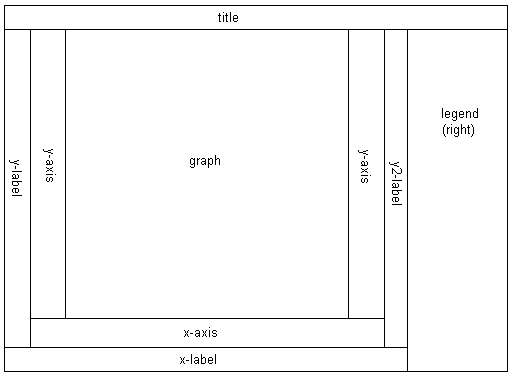
\includegraphics[scale=0.4]{Elemente.png}
  \end{center}
  \caption{Layout Elements of a chart}
  \label{fig:Elemente}
\end{figure}

The graph area in the middle is drawn by the subclass, all the other
elements are drawn by \class{Chart::Base}. But some classes do not need
all of those elements, or they may need additional elements. The
\class{Chart::Base} methods producing these elements have then to be
overwritten in the respective subclass. For example, class
\class{Chart::Pie} needs no axes, so the methods for drawing these in
file Base.pm are overwritten by methods in class \class{Chart::Pie}; in
this case, no axes are drawn. Furthermore, the legend in a pie chart is
slightly different. Therefore, Pie.pm has its own methods for drawing
the legends. All these rules are managed by \class{Chart}, so you do not
have to attend to it.

\class{Chart} uses Lincoln Stein's GD module for all its graphics
primitives calls. So you need an installed version of GD.pm to use
\class{Chart}. This module is available in the CPAN online archive at
\texttt{http://www.cpan.org/}, just like \class{Chart} itself.
\index{GD (module by Lincoln Stein)}

The table lists all attributes that are currently used within the Chart
package. It shows which of the concrete subclasses uses each attribute.

{
\begin{sidewaystable}
\tiny
\begin{tabular}{|l|c|c|c|c|c|c|c|c|c|c|c|c|c|}
\hline
Attribute & Bars& Composite& Direction& ErrorBars& HorizontalBars& Lines& LinesPoints& Mountain& Pareto& Pie& Points& Split& StackedBars \\
\hline
angle\_interval        &   &   & X &   &   &   &   &   &   &   &   &   &   \\
arrow                  &   &   & X &   &   &   &   &   &   &   &   &   &   \\
brush\_size            &   &   & X & X &   & X & X &   &   &   &   &   &   \\
brush\_size1           &   & X &   &   &   &   &   &   &   &   &   &   &   \\
brush\_size2           &   & X &   &   &   &   &   &   &   &   &   &   &   \\
colors                 & X & X & X & X & X & X & X & X & X & X & X & X & X \\
composite\_info        &   & X &   &   &   &   &   &   &   &   &   &   &   \\
custom\_x\_ticks       & X & X & X & X & X & X & X & X & X & X & X & X & X \\
f\_x\_tick             & X & X & X & X & X & X & X & X & X & X & X & X & X \\
f\_y\_tick             & X & X & X & X & X & X & X & X & X & X & X & X & X \\
f\_y\_tick1            &   & X &   &   &   &   &   &   &   &   &   &   &   \\
f\_y\_tick2            &   & X &   &   &   &   &   &   &   &   &   &   &   \\
graph\_border          & X & X & X & X & X & X & X & X & X & X & X & X & X \\
grey\_background       & X & X & X & X & X & X & X & X & X & X & X & X & X \\
grid\_lines            & X & X & X & X & X & X & X & X & X & X & X & X & X \\
imagemap               & X & X & X & X & X & X & X & X & X & X & X & X & X \\
include\_zero          & X & X & X & X & X & X & X & X & X & X & X & X & X \\
integer\_ticks\_only   & X & X & X & X & X & X & X & X & X & X & X & X & X \\
interval               &   &   &   &   &   &   &   &   &   &   &   & X &   \\
interval\_ticks        &   &   &   &   &   &   &   &   &   &   &   & X &   \\
label\_font            & X & X & X & X & X & X & X & X & X & X & X & X & X \\
label\_values          &   &   &   &   &   &   &   &   &   & X &   &   &   \\
legend                 & X & X & X & X & X & X & X & X & X & X & X & X & X \\
legend\_example\_height&   & X &   &   &   &   &   &   &   &   &   &   &   \\
legend\_example\_size  & X & X & X & X & X & X & X & X & X & X & X & X & X \\
legend\_font           & X & X & X & X & X & X & X & X & X & X & X & X & X \\
legend\_label\_values  &   &   &   &   &   &   &   &   &   & X &   &   &   \\
legend\_labels         & X & X & X & X & X & X & X & X & X & X & X & X & X \\
legend\_lines          &   &   &   &   &   &   &   &   &   & X &   &   &   \\
line                   &   &   & X &   &   &   &   &   &   &   &   &   &   \\
max\_circles           &   &   & X &   &   &   &   &   &   &   &   &   &   \\
max\_val               & X & X & X & X & X & X & X & X & X & X & X & X & X \\
max\_val1              &   & X &   &   &   &   &   &   &   &   &   &   &   \\
max\_val2              &   & X &   &   &   &   &   &   &   &   &   &   &   \\
max\_x\_ticks          & X & X & X & X & X & X & X & X & X & X & X & X & X \\
max\_y\_ticks          & X & X & X & X & X & X & X & X & X & X & X & X & X \\
min\_circles           &   &   & X &   &   &   &   &   &   &   &   &   &   \\
min\_val               & X & X & X & X & X & X & X & X & X & X & X & X & X \\
min\_val1              &   & X &   &   &   &   &   &   &   &   &   &   &   \\
min\_val2              &   & X &   &   &   &   &   &   &   &   &   &   &   \\
min\_x\_ticks          & X & X & X & X & X & X & X & X & X & X & X & X & X \\
min\_y\_ticks          & X & X & X & X & X & X & X & X & X & X & X & X & X \\
no\_cache              & X & X & X & X & X & X & X & X & X & X & X & X & X \\
pairs                  &   &   & X &   &   &   &   &   &   &   &   &   &   \\
png\_border            & X & X & X & X & X & X & X & X & X & X & X & X & X \\
point                  &   &   & X &   &   &   &   &   &   &   &   &   &   \\
precision              & X & X & X & X & X & X & X & X & X & X & X & X & X \\
pt\_size               &   &   & X & X &   &   & X &   &   &   & X &   &   \\
ring                   &   &   &   &   &   &   &   &   &   & X &   &   &   \\
same\_error            &   &   &   & X &   &   &   &   &   &   &   &   &   \\
same\_y\_axes          &   & X &   &   &   &   &   &   &   &   &   &   &   \\
scale                  &   &   &   &   &   &   &   &   &   &   &   & X &   \\
skip\_int\_ticks       & X & X & X & X & X & X & X & X & X & X & X & X & X \\
skip\_x\_ticks         & X & X & X & X & X & X & X & X & X & X & X & X & X \\
skip\_y\_ticks         &   &   &   &   & X &   &   &   &   &   &   &   &   \\
sort                   &   &   & X & X &   & X & X &   & X &   & X & X &   \\
spaced\_bars           & X &   &   &   & X &   &   &   & X &   &   &   & X \\
start                  &   &   &   &   &   &   &   &   &   &   &   & X &   \\
stepline               &   &   &   &   &   & X & X &   &   &   &   &   &   \\
stepline\_mode         &   &   &   &   &   & X & X &   &   &   &   &   &   \\
sub\_title             & X & X & X & X & X & X & X & X & X & X & X & X & X \\
text\_space            & X & X & X & X & X & X & X & X & X & X & X & X & X \\
tick\_label\_font      & X & X & X & X & X & X & X & X & X & X & X & X & X \\
tick\_len              & X & X & X & X & X & X & X & X & X & X & X & X & X \\
title                  & X & X & X & X & X & X & X & X & X & X & X & X & X \\
title\_font            & X & X & X & X & X & X & X & X & X & X & X & X & X \\
transparent            & X & X & X & X & X & X & X & X & X & X & X & X & X \\
x\_grid\_lines         & X & X & X & X & X & X & X & X & X & X & X & X & X \\
x\_label               & X & X & X & X & X & X & X & X & X & X & X & X & X \\
x\_ticks               & X & X & X & X & X & X & X & X & X & X & X & X & X \\
xlabels                &   &   &   & X &   & X & X &   &   &   & X &   &   \\
xrange                 &   &   &   & X &   & X & X &   &   &   & X &   &   \\
xy\_plot               &   &   &   & X &   & X & X &   &   &   & X &   &   \\
y\_axes                & X &   &   & X & X &   & X & X & X &   & X & X & X \\
y\_grid\_lines         & X & X & X & X & X & X & X & X & X & X & X & X & X \\
y\_label               & X & X & X & X & X & X & X & X & X & X & X & X & X \\
y\_label2              & X & X & X & X & X & X & X & X & X & X & X & X & X \\
y\_ticks               & X & X & X & X & X & X & X & X & X & X & X & X & X \\
y\_ticks1              &   & X &   &   &   &   &   &   &   &   &   &   &   \\
y\_ticks2              &   & X &   &   &   &   &   &   &   &   &   &   &   \\
ylabel2                & X & X & X & X & X & X & X & X & X & X & X & X & X \\
\hline
\end{tabular}
\end{sidewaystable}
}


%\section{Example}

\section{Chart::Base}
\herv{Name:} Chart::Base\\ \\
\herv{File:} Base.pm\\ \\
\herv{Requires:}GD, Carp, FileHandle\\ \\
\herv{Description:} \fett{Base} is the \fett{abstract superclass} of the modules: Bars, Composite, Direction, ErrorBars, HorizontalBars, Lines, LinesPoints, Mountain, Pareto, Pie, Points, Split, StackedBars\\
The class Base provides all public methods and most of the attributs of a chart object.\\
\\
\herv{Constructor:} An instance of a chart object can be created with the constructor new():\\
\fett{\$obj = Chart::\kursiv{Type}->new();}\\
\fett{\$obj = Chart::\kursiv{Type}->new(\kursiv{width}, \kursiv{height});}\\
\\
\kursiv{Type} means the type of chart it returns, i.e. Chart::Bars returns a chart with bars.\\
If \fett{new} has no arguments, the constructor returns an object with the size 300x400 pixels. If new has two arguments \kursiv{width} and \kursiv{height}, it returns a chart object with the desired size. \\ 
\\ 
\label{methods}\herv{Methods:}\\
\\
\fett{\$obj->add\_dataset(@array);}\\ \fett{\$obj->add\_dataset($\backslash$@array\_ref);}\\
Adds a dataset to the object. The parameter is an array or a reference to an array. Generally the first added array are interpreted by chart as the x-tick labels. The following arrays should include the data points. For example if the first call with an bars object is\\
\\
\kursiv{\$obj->add\_dataset('Harry', 'Sally');}  and the second call is\\ \kursiv{\$obj->add\_dataset(5, 8);}\\
\\
then chart will draw a picture with two bars and label them with Harry and Sally.\\ \\
Some modules handle it a little bit different. Look at the respective description of the module to get more information.\\
There are also differences if you want to use the \fett{xy\_plot} option, to create a xy-graph. \\
\\
\\
\fett{\$obj->add\_pt(@array);} \\ \fett{\$obj->add\_pt($\backslash$@array\_ref);}\\
This is another method to add data to a chart object. An argument can be an array or a reference to an array. If you use this method, chart wants the complete data of one data point.\\
For example\\
\\
\kursiv{\$obj->add\_pt('Harry', 5);}\\ 
\kursiv{\$obj->add\_pt('Sally', 8);}\\
\\
would create the same graph as the example for add\_dataset.\\
\\
\\
\fett{\$obj->add\_datafile( "file", \kursiv{type} );} \\
\fett{\$obj->add\_datafile( \$filehandle, \kursiv{type} );} \\
This method adds a complete data file to the chart object.\\
\kursiv{Type} can be 'set' or 'pt'. If the parameter is 'set' then one line in the data file has to be a complete data set. The values of the set has to be separated by whitespaces. For Example the file looks like this:\\
\\
Harry  Sally\\
3      8\\
2      1\\
\\
If the parameter is 'pt' the lines of the file have to look like the parameter arrays of the add\_pt method. Which means the line includes all values of one data point, also separated by whitespaces. For Example:\\
\\
Harry 3 2\\
Sally 8 1\\
\\
\\
\fett{\$obj->get\_data();} \\
If you want a copy of the data that has been added so far, make a call to the get\_data method like so:\\
\\
\kursiv{\$dataref = \$obj->get\_data();}\\
\\
It returns a reference to an array of references to datasets. For Example, you can get the x-tick labels this way:\\
\kursiv{@x\_labels = @\{\$dataref->[0]\};}\\
\\
\\ 
\fett{\$obj->clear\_data();} \\
This is the method to remove all data that may have been entered before.\\
\\
\\
\fett{\$obj->set( \kursiv{attribut 1} => \kursiv{value 1}, ... ,\mbox{\kursiv{attribute n} => \kursiv{value n}} );}\\
\fett{\$obj->set( \%hash );}\\
\fett{\$obj->set( \kursiv{attribut 1}, \kursiv{value 1}, ... ,\mbox{\kursiv{attribute n}, \kursiv{value n}} );}\\
\fett{\$obj->set( @array );}\\
Use this method to change the attributes of the chart object. Set looks for a hash of keys and values or an array of keys and values.\\
For Example\\
\\
\kursiv{\$obj->set( 'title' => 'The title of the image');}\\
\\
would set the title. The same job would do:\\
\\
\kursiv{\%hash = ('title' => 'The title of the image');}\\ 
\kursiv{\$obj->set( \%hash);}\\
\\
\\
\fett{\$obj->png( "file" );} \\
\fett{\$obj->png( \$filehandle );} \\
\fett{\$obj->png( FILEHANDLE );} \\
\fett{\$obj->png( "file", $\backslash$@data );}\\
This method creates the png file. The file parameter can be, the file name, a reference to a filehandle or a filehandle itself. If the file doesn't exist, chart will create a file for you. If there is already a file, chart will overwrite this file.\\
You can also add the data to the chart object in the png method. The @data array should contain references to arrays of data, with the first array reference pointing to an array with x-tick labels. @data could look like this:\\
\\
\kursiv{@data = (['Harry', 'Sally'], [5, 8], [50, 80]);}\\
\\
This would set up an graph with two datasets, and three data points in these sets.\\
\\
\\
\fett{\$obj->jpeg( "file" );} \\
\fett{\$obj->jpeg( \$filehandle );} \\
\fett{\$obj->jpeg( FILEHANDLE );} \\
\fett{\$obj->jpeg( "file", $\backslash$@data );}\\
These are the methods to create jpeg files. They work similar like the png() method. \\
\\
\\
\fett{\$obj->cgi\_png();} \\
\fett{\$obj->cgi\_jpeg();} \\
With the cgi methods you can create dynamic images for your web site. The cgi methods will print the chart, along with the appropriate http header to stdout, allowing you to call chart-generating scripts directly from your html pages (ie. with a <img scr=image.pl>HTML tag).\\
\\
\\
\fett{\$obj->imagemap\_dump();} \\ 
Chart can also return the pixel positioning information so that you can create image maps from the files Chart generates. Simply set the 'imagemap' option to 'true' before you generate the file, then call the imagemap\_dump method to retrieve the information. A structure will be returned almost identical to the @data array described above to pass the data into Chart.\\
\\
\kursiv{\$imagemap\_data = \$obj->imagemap\_dump();}\\
\\
Instead of single data values, you will be passed references to arrays of pixel information. For Bars, HorizontalBars, Pareto and StackedBars charts, the arrays will contain two x-y pairs (specifying the upper left and the lower right corner of the bar), like so\\
\\
\kursiv{( \$x1, \$y1, \$x2, \$y2 ) = @\{ \$imagemap\_data->[\$dataset][\$datapoint] \};}\\
\\ 
For Lines, Points, LinesPoints and Split, the arrays will contain a single xy-pair (specifying the center of the point), like so\\
\\
\kursiv{( \$x, \$y) = @\{ \$imagemap\_data->[\$dataset][\$datapoint] \};}\\
\\
A few caveats apply here. First of all, Chart uses the GD-module by Lincoln Stein to draw lines, circles, strings, and so on. GD treats the upper-left corner of the png/jpeg as the (0,0) point, so positives y values are measured from the top of the png/jpeg, not the bottom. Second, these values will mostly contain long decimal values. GD, of course, has to truncate these to single pixel values. In a worst-case scenario, this will result an error of one pixel on your imagemap. If this is really an issue, your only option is to experiment with it, or to contact Lincoln Stein and ask him. Third, please remember that the 0th dataset will be empty, since that's the place in the @data array for the data point labels.\\
\\
\\   
\label{options}\herv{Attributes/Options:} These are the options which have effects on all types of chart:
\begin{description}
\item ['transparent']Makes the background of the image transparent if set to 'true'. Useful for making web page images. It doesn't work for all browsers. Defaults to false.
\item ['png\_border']Sets the number of pixels used as a border between the graph and the edges of the png/jpeg. Defaults to 10.
\item ['graph\_border']Sets the number of pixels used as a border between the title/labels and the actual graph within the png/jpeg.  Defaults to 10.
\item['text\_space']Sets the amount of space left on the sides of text, to make it more readable.  Defaults to 2.
\item['title']Tells Chart what to use for the title of the graph.  If empty, no title is drawn.  It recognizes '$\backslash$n' as a newline, and acts accordingly. Remember, if you want to use normal quotation marks instead of single quotation marks then you have to quote "`$\backslash\backslash$n"'. Default is empty.
\item['sub\_title']Writes a sub-title under the title in smaller letters.
\item['x\_label']Tells Chart what to use for the x-axis label.  If empty, no label is drawn.  Default is empty.
\item['y\_label', 'y\_label2']Tells Chart what to use for the y-axis labels.  If empty, no label is drawn.  Default is empty.
\item['legend']Specifies the placement of the legend.  Valid values are 'left', 'right', 'top', 'bottom'.  Setting this to 'none' tells chart not to draw a legend.  Default is 'right'.
\item['legend\_labels']Sets the values for the labels for the different datasets. Should be assigned a reference to an array of labels.  For example,\\
\\
@labels = ('foo', 'bar');\\
\$obj->set ('legend\_labels' => $\backslash$@labels);\\
\\
Default is empty, in which case 'Dataset 1', 'Dataset 2', etc. are used as the labels.
\item['tick\_len']Sets the length of the x- and y-ticks in pixels.  Default is 4.
\item['x\_ticks']Specifies how to draw the x-tick labels.  Valid values are 'normal', 'staggered' (staggers the labels vertically), and 'vertical' (the labels are draw upwards).  Default is 'normal'.
\item['min\_y\_ticks']Sets the minimum number of y\_ticks to draw when generating a scale. Default is 6, The minimum is 2.
\item['max\_y\_ticks']Sets the maximum number of y\_ticks to draw when generating a scale. Default is 100. This limit is used to avoid plotting an unreasonably large number of ticks if non-round values are used for the min\_val and max\_val.\\
\\
The value for 'max\_y\_ticks' should be at least 5 times larger than 'min\_y\_ticks'.
\item['max\_x\_ticks', 'min\_x\_ticks'] Works similar as 'max\_y\_ticks' and 'min\_y\_ticks'. Of course, it works only for xy-plots! 
\item['integer\_ticks\_only']Specifies how to draw the x- and y-ticks: as floating point ('false', '0') or as integer numbers ('true', 1). If you want integer ticks, it is maybe better to set the option 'precision' at zero. Default: 'false'
\item['skip\_int\_ticks']If 'integer\_ticks\_only' was set to 'true' the labels and ticks at the y-axis will be drawn every nth tick. Of course in HorizontalBars it affects the x-axis. Default to 1, no skipping.
\item['precision'] Sets the number of numerals after the decimal point. Affects in most cases the y-axis. But also the x-axis if 'xy\_plot' is set and the labels in a pie chart. Defaults to 3.
\item['max\_val']Sets the maximum y-value on the graph, overriding the normal autoscaling.  Does not work for a Split chart. Default is undef.
\item['min\_val']Sets the minimum y-value on the graph, overriding the normal autoscaling.  Does not work for a Split chart. Default is undef.\\
\\
Caution should be used when setting 'max\_val' and 'min\_val' to floating point or non-round numbers. This is because the scale must start \& end on a tick, ticks must have round-number intervals, and include round numbers.\\
\\
Example: Suppose your dataset has a range of 35-114 units, If you specify them as the 'min\_val' \& 'max\_val', The y\_axis will be plot with 80 ticks every 1 unit.. If no 'min\_val' \& 'max\_val', the system will autoscale the range to 30-120 with 10 ticks every 10 units.\\
\\
If the 'min\_val' \& 'max\_val' are specified to exesive precision, they may be overiden by the system, plotting a maximum 'max\_y\_ticks' ticks. 
\item['include\_zero']If 'true', forces the y-axis to include zero if it is not in the dataset range. Default is 'false'.\\
\\
In general, it is better to use this, than to set the 'min\_val' if that is all you want to achieve.
\item['skip\_x\_ticks']Sets the number of x-ticks and x-tick labels to skip.  (ie. if 'skip\_x\_ticks' was set to 4, Chart would draw every 4th x-tick and x-tick label).  Default is undef.
\item['custom\_x\_ticks']This option allows you to specify exactly which x-ticks and x-tick labels should be drawn. It should be assigned a reference to an array of desired ticks.  Just remember that I'm counting from the 0th element of the array.  (e.g., if 'custom\_x\_ticks' is assigned [0,3,4], then the 0th, 3rd, and 4th x-ticks will be displayed) It doesn't work for Split, HorizontalBars and Pie.
\item['f\_x\_tick']Needs a reference to a function which uses the x-tick labels generated by the @data->[0] as the argument. The result of this function can reformat the labels. For instance\\
\\
\$obj -> set ('f\_x\_tick' => $\backslash$\&formatter );\\
\\
An example for the function formatter: x labels are seconds since an event. The referenced function can transform this seconds to hour, minutes and seconds.
\item['f\_y\_tick']The same situation as for 'f\_x\_tick' but now used for y labels.
\item['colors']This option lets you control the colors the chart will use.  It takes a reference to a hash.  The hash should contain keys mapped to references to arrays of rgb values.  For instance,\\
\\
\$obj->set('colors' => {'background' => [255,255,255]});\\
\\
sets the background color to white (which is the default).  Valid keys for this hash are\\
\\
'background' (background color for the png)\\
'title' (color of the title)\\
'text' (all the text in the chart)\\
'x\_label' (color of the x axis label)\\ 
'y\_label' (color of the first y axis label)\\
'y\_label2' (color of the second y axis label)\\
'grid\_lines' (color of the grid lines)\\
'x\_grid\_lines' (color of the x grid lines - for x axis ticks)\\
'y\_grid\_lines' (color of the y grid lines - for to left y axis ticks)\\
'y2\_grid\_lines' (color of the y2 grid lines - for right y axis ticks)\\
'dataset0'..'dataset63' (the different datasets)\\
'misc' (everything else, e.g. ticks, box around the legend)\\
\\
NB. For composite charts, there is a limit of 8 datasets per component. The colors for 'dataset8' through 'dataset15' become the colors for 'dataset0' through 'dataset7' for the second component chart.
\item['title\_font'] This option changes the font of the title. The key has to be a Gd font. e.g. GD::Font->Large 
\item['label\_font'] This option changes the font of the labels. The key has to be a Gd font. 
\item['legend\_font'] This option changes the font of the text of the legend. The key has to be a Gd font. 
\item['tick\_label\_font'] This option changes the font of the ticks. The key has to be a Gd font. 
\item['grey\_background']Puts a nice soft grey background on the actual data plot when set to 'true'.  Default is 'true'.
\item['x\_grid\_lines']Draws grid lines matching up to x ticks if set to 'true'. Default is 'false'.
\item['y\_grid\_lines']Draws grid lines matching up to y ticks if set to 'true'. Default is 'false'.
\item['grid\_lines']Draws grid lines matching up to x and y ticks if set to 'true'. Default is 'false'. 
\item['imagemap']Lets Chart know you're going to ask for information about the placement of the data for use in creating an image map from the png. This information can be retrieved using the imagemap\_dump() method.  NB. that the imagemap\_dump() method cannot be called until after the Chart has been generated (e.g. using the png() or cgi\_png() methods).
\item['ylabel2']The label for the right y-axis (the second component chart).  Default is undef.
\item['no\_cache']Adds Pragma: no-cache to the http header. Be careful with this one, as Netscape 4.5 is unfriendly with POST using this method.
\item['legend\_example\_size'] Sets the length of the example line in the legend. Defaults to 20.
\end{description}

 
%
% bars.tex
%
\section{Chart::Bars}
\index{Chart::Bars}
\name{Chart::Bars}
\file{Bars.pm}
\requires{Chart::Base, GD, Carp, FileHandle}
\begin{Description} 
   \class{Bars} is a \textbf{subclass} of the module \module{Chart::Base}.
   The class \class{Bars} creates a chart with bars.
\end{Description}

\parindent 0pt{\large Example:}
\begin{figure}[h]
 	\begin{center}
		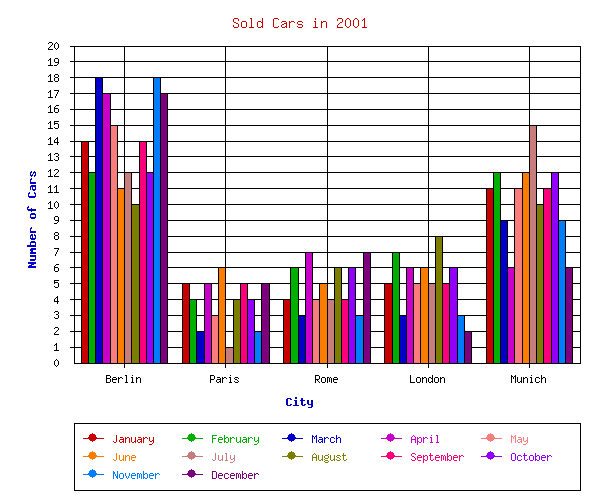
\includegraphics[scale=0.4]{d_bars.png}
	\end{center}
	\caption{Bars chart}
	\label{fig:bars}
\end{figure}

\begin{verbatim}
use Chart::Bars;

$g = Chart::Bars->new(600,500);

$g->add_dataset ('Berlin', 'Paris', 'Rome', 'London', 'Munich');
$g->add_dataset (14, 5, 4, 5, 11);
$g->add_dataset (12, 4, 6, 7, 12);
$g->add_dataset (18, 2, 3, 3, 9);
$g->add_dataset (17, 5, 7, 6, 6);
$g->add_dataset (15, 3, 4, 5, 11);
$g->add_dataset (11, 6, 5, 6, 12);
$g->add_dataset (12, 1, 4, 5, 15);
$g->add_dataset (10, 4, 6, 8, 10);
$g->add_dataset (14, 5, 4, 5, 11);
$g->add_dataset (12, 4, 6, 6, 12);
$g->add_dataset (18, 2, 3, 3, 9);
$g->add_dataset (17, 5, 7, 2, 6);

%hash = ('title' => 'Sold Cars in 2001',
         'text_space' => 5,
         'grey_background' => 'false',
         'integer_ticks_only' => 'true',
         'x_label' => 'City',
         'y_label' => 'Number of Cars',
         'legend' => 'bottom',
         'legend_labels' => ['January' , 'February' , 'March', 'April',
                             'May', 'June', 'July', 'August', 'September',
                             'October', 'November', 'December'],
         'min_val' => 0,
         'max_val' => 20,
         'grid_lines' =>'true',
         'colors' => {'title' => 'red',
                      'x_label' => 'blue',
                      'y_label' => 'blue'} );

$g->set (%hash);

$g->png ("bars.png");

\end{verbatim}

\begin{Constructor} 
An instance of a bars chart object can be created with the constructor new():
\begin{quote}
\parindent 0pt
\fett{\$obj = Chart::Bars->new();}\\
\fett{\$obj = Chart::Bars->new(\kursiv{width}, \kursiv{height});}\\
\end{quote}

If \textit{new()} has no arguments, 
the constructor returns an image with the size 300x400 pixels. 
If new has two arguments \parameter{width} and \parameter{height}, 
it returns an image with the desired size.
\end{Constructor}

\Methods
\method{All universally valid methods, see page \pageref{methods} of 
class \class{Chart::Base}.}\\[\parabstand]
%
\Attributes
All universal valid options, see page \pageref{options}. \\
In addition, the following options for this class are defined:
\begin{description}
\item['y\_axes'] Tell chart where to place the y-axis. 
                 Valid values are 'left', 'right' and 'both'. Defaults to 'left'.
                 
\item['spaced\_bars'] Leaves space between the groups of bars at each data point when set to 'true'.  
             This just makes it easier to read a bar chart.  Default is 'true'.
\end{description}
\section{Chart::Composite}
\herv{Name:} Chart::Composite\\ \\
\herv{File:} Composite.pm\\ \\
\herv{Requires:}Chart::Base, GD, Carp, FileHandle\\ \\
\herv{Description:} \fett{Composite} is a \fett{subclass} of Chart::Base.\\
The class Composite creates a two component chart with two types of chart. For example you can create a two component chart with bars and lines. Just set the option 'composite\_info'! A composite chart doesn't make sense with all types of chart. But it works pretty good with Lines, Points, LinesPoints and Bars.\\ 
\\
\herv{Example:}
\begin{figure}[h]
	\begin{center}
		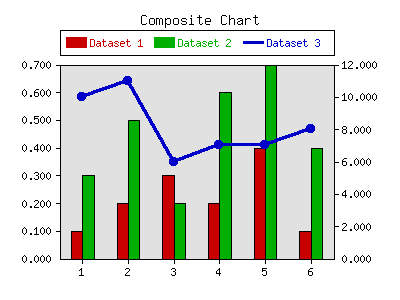
\includegraphics[scale=0.6]{composite.png}
	\end{center}
	\caption{Composite chart}
	\label{fig:composite}
\end{figure}
\begin{verbatim}
use Chart::Composite;

$g = Chart::Composite->new;

$g->add_dataset (1 , 2, 3, 4, 5, 6);
$g->add_dataset (0.1, 0.2, 0.3, 0.2, 0.4, 0.1);
$g->add_dataset (0.3, 0.5, 0.2, 0.6, 0.7, 0.4);
$g->add_dataset (10, 11, 6, 7, 7, 8);

$g->set('title' => 'Composite Chart',
        'composite_info' => [ ['Bars', [1,2]],
                               ['LinesPoints', [3]] ] );
$g->set( 'include_zero' => 'true');

$g->png("composite.png");
\end{verbatim}
\herv{Constructor:} An instance of a Composite object can be created with the constructor new():\\
\fett{\$obj = Chart::Composite->new();}\\
\fett{\$obj = Chart::Composite->new(\kursiv{width}, \kursiv{height});}\\
\\
If \fett{new} has no arguments, the constructor returns an image with the size 300x400 pixels. If new has two arguments \kursiv{width} and \kursiv{height}, it returns an image with the desired size. \\ 
\\ 
\herv{Methods:}All universally valid methods, see page \pageref{methods}: Chart::Base. \\
\\
\herv{Attributes/Options:} All universally valid options, see page \pageref{options}. Also available, these special options:
\begin{description}
\item['composite\_info']This option is only used for composite charts.  It contains the information about which types to use for the two component charts, and which datasets belong to which component chart. It should be a reference to an array of array references, containing information like the following\\
\$obj->set ('composite\_info' => [ ['Bars', [1,2]],                      ['Lines', [3,4] ] ]);\\
\\
This example would set the two component charts to be a bar chart and a line chart. It would use the first two data sets for the bar chart (note that the numbering starts at 1, not zero like most of the other numbered things in Chart), and the second two data sets for the line chart. The default is undef.\\
\\
NB. Chart::Composite can only do two component charts.
\item['min\_val1', 'min\_val2']Only for composite charts, these options specify the minimum y-value for the first and second components respectively. Both default to undef.
\item['max\_val1', 'max\_val2']Only for composite charts, these options specify the maximum y-value for the first and second components respectively. Both default to undef.
\item['y\_ticks1', 'y\_ticks2']The number of y ticks to use on the first and second y-axis on a composite chart.  Please note that if you just set the 'y\_ticks' option, both axes will use that number of y ticks. Both default to undef.
\item['same\_y\_axes']Forces both component charts in a composite chart to use the same maximum and minimum y-values if set to 'true'. This helps to keep the composite charts from being too confusing. Default is undef.
\end{description}
\section{Chart::Direction}
\herv{Name:} Chart::Direction\\ \\
\herv{File:} Direction.pm\\ \\
\herv{Requires:}Chart::Base, GD, Carp, FileHandle\\ \\
\herv{Description:} \fett{Direction} is a \fett{subclass} of Chart::Base.\\
The class Direction creates a diagram for polar coordinates.\\
Direction plots data, which is specified by angle (eg. wind direction) and value (eg. wind strength). The first dataset to add is a set of angles in degrees. The second set is a set of values. Following sets have no influence.\\ 
In the default case, direction will draw a point chart. You can also get a lines chart by turning the option 'point' to 'false' and the option 'line' to 'true'. If you want a linespoint chart, then 'point' and 'line' has to be 'true'. Additionally chart plots arrows from the center to the point or to the end of the line, if the option 'arrow' is set to 'true'.\\
\\
\herv{Example:}
\begin{figure}[h]
	\begin{center}
		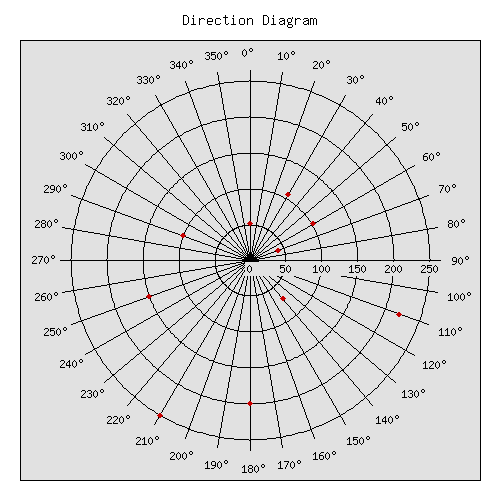
\includegraphics[width = 8cm, height =8cm]{ort.png}
	\end{center}
	\caption{Direction chart}
	\label{fig:direction}
\end{figure}
\begin{verbatim}
use Chart::Direction;
$g = Chart::Direction->new(500,500);

$g->add_dataset(0, 180, 290, 70, 60, 250, 210, 30, 110, 140 );
$g->add_dataset(50, 200, 100, 40, 100, 150, 250, 105, 220, 70);

%hash = ( 'title' => 'Direction Diagram',
          'legend' => 'none',
          'precision' => 0,
          'angle_interval' => 10,
          'pt_size' => 10);
      
$g->set(%hash);
$g->png("Grafiken/ort.png");
\end{verbatim}
\herv{Constructor:} An instance of a direction chart object can be created with the constructor new():\\
\fett{\$obj = Chart::Direction->new();}\\
\fett{\$obj = Chart::Direction->new(\kursiv{width}, \kursiv{height});}\\
\\
If \fett{new} has no arguments, the constructor returns an image with the size 300x400 pixels. If new has two arguments \kursiv{width} and \kursiv{height}, it returns an image with the desired size. \\ 
\\ 
\herv{Methods:}All universally valid methods, see page \pageref{methods}: Chart::Base. \\
\\
\herv{Attributes/Options:} All universally valid options, see page \pageref{options}, apart from the Options, that have effects on the axes, like 'custom\_x\_ticks', 'x\_ticks' and so on. Also available, these special options:
\begin{description}
\item['point'] Indicates to draw points, representing the data values. 'true' or 'false' possible, per default 'true'.
\item['line'] Connects the points with lines if set to 'true'. Defaults to 'false'.
\item['arrow'] Draws an arrow from the center of the chart to the point, if set to 'true', per default 'false'.
\item['angle\_interval'] This option tells Chart, how many angle lines should be drawn. It is the difference between two angle lines. The default value is 30, which means that a line will be drawn every 30 degrees. There are not all values allowed. Valid Values are: 0, 5, 10, 15, 20, 30, 45 and 90. If you choose 0, Chart will draw no line.  
\item['pt\_size']Sets the radius of the points in pixels. Default is 18.
\item['brush\_size']Sets the width of the lines in pixels. Default is 6.
\item['min\_circles'] Sets the minimum number of circles to draw when generating a scale. Default is 4, the minimum is 2.
\item['max\_circles']Sets the maximum number of circles to draw when generating a scale. Default is 100. This limit is used to avoid plotting an unreasonably large number of ticks if non-round values are used for the min\_val and max\_val.\\
The value for 'max\_circles' should be at least 5 times larger than 'min\_circles'.
\end{description}
%
% error.tex
%
\section{Chart::ErrorBars}
\name{Chart::ErrorBars}
\file{ErrorBars.pm}
\requires{Chart::Base, GD, Carp, FileHandle}

\begin{Description} 
\class{ErrorBars} is a subclass of \class{Chart::Base}.
The class \class{ErrorBars} creates a point chart with error bars.\\
Chart expects the error values within the data array. 
By use of the \method{add\_dataset()} method the error values are the next two sets after the y values. The first set after the y values has to be a set values for the upper error bars. 
The next set is an array of the down errors.\\
If you want to use the same value for the up and down error, then you have to set the 
'same\_error' option to 'true'. In this case only one set after the y values is interpreted 
as a set of errors.\\
Of course, it's also possible to use the \method{add\_pt()} method in a respective way.
\end{Description}

\parindent 0pt{\large Example:}
\begin{figure}[h]
	\begin{center}
		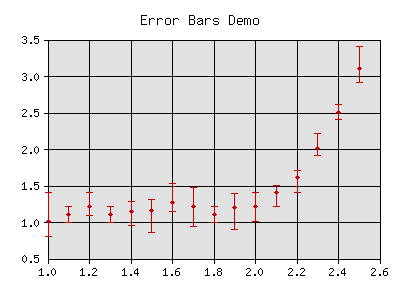
\includegraphics[scale=0.7]{error.png}
	\end{center}
	\caption{Error bars chart}
	\label{fig:error}
\end{figure}

\begin{verbatim}
use Chart::ErrorBars;
$g = Chart::ErrorBars->new();

#the x values
$g->add_dataset(qw(1   1.1  1.2  1.3  1.4  1.5  1.6  1.7  1.8  1.9  2
                   2.1 2.2  2.3  2.4  2.5));
#the y values
$g->add_dataset(qw(1   1.1  1.2  1.1  1.14 1.15 1.26 1.2  1.1  1.19 1.2
                   1.4 1.6  2.0  2.5  3.1));
#the up errors
$g->add_dataset(qw(0.4 0.1  0.2  0.1  0.14 0.15 0.26 0.27 0.1  0.19 0.2
                   0.1 0.1  0.2  0.1  0.3));
#the down errors
$g->add_dataset(qw(0.2 0.11 0.12 0.11 0.2  0.3  0.12 0.27 0.11 0.3  0.2
                   0.2 0.2  0.1  0.1  0.2));
                   
$g->set( 'xy_plot' => 'true',
         'precision' => 1,
         'pt_size' =>10, 'brush_size' => 2,
         'legend' => 'none',
         'title' => 'Error Bars Demo',
         'grid_lines' => 'true');

$g->png("errorbars.png");
\end{verbatim}

\begin{Constructor}
An instance of a error bars chart object can be created with the constructor new():
\begin{quote}
\parindent 0pt
\fett{\$obj = Chart::ErrorBars->new();}\\
\fett{\$obj = Chart::ErrorBars->new(\parameter{width}, \parameter{height});}
\end{quote}

If \textit{new()} has no arguments, the constructor returns an image with the size 300x400 pixels. If \textit{new()} has two arguments \parameter{width} and \parameter{height}, 
it returns an image with the desired size.
\end{Constructor}


\Methods
\method{All universal valid methods, see page \pageref{methods}: \class{Chart::Base}.} \\[\parabstand]


\Attributes
All universally valid options, see page \pageref{options}. Also available these special options:
\begin{description}
\item['same\_error'] Tells chart that you want to use the same error value of a data point 
     if set to true. 
     Then you have to add just one set of error values. Defaults to 'false'.
     
\item['y\_axes'] Tells chart where to place the y-axis. 
     Valid values are 'left', 'right' and 'both'. Defaults to 'left'.

\item['pt\_size']Sets the radius of the points in pixels. Default is 18.

\item['brush\_size']Sets the width of the lines in pixels. Default is 6.

\item['xy\_plot']Forces Chart to plot a x-y-graph, 
      which means that the x-axis is also numeric if set to 'true'. 
      Very useful for plots of mathematical functions. Defaults to 'false'.

\item['sort']Sorts the data of a x-y-graph ascending if set to 'true'. 
      Should be set if the added data isn't sorted. Defaults to 'false'. 
\end{description}

\section{Chart::HorizontalBars}
\herv{Name:} Chart::HorizontalBars\\ \\
\herv{File:} HorizontalBars.pm\\ \\
\herv{Requires:}Chart::Base, GD, Carp, FileHandle\\ \\
\herv{Description:} \fett{HorizontalBars} is a \fett{subclass} of Chart::Base.\\
The class HorizontalBars creates a chart with bars, that run horizontal.\\
\\
\herv{Example:}
\begin{figure}[h]
	\begin{center}
		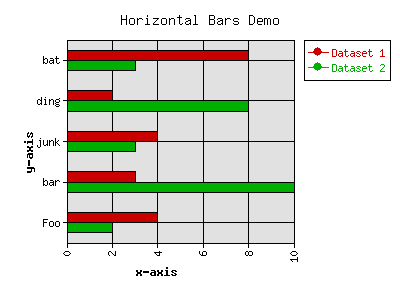
\includegraphics[scale=0.7]{d_hbars4.png}
	\end{center}
	\caption{Chart with horizontal bars}
	\label{fig:hbars}
\end{figure}
\begin{verbatim}
use Chart::HorizontalBars;

$g = Chart::HorizontalBars->new();
$g->add_dataset ('Foo', 'bar', 'junk', 'ding', 'bat');
$g->add_dataset (4, 3, 4, 2, 8);
$g->add_dataset (2, 10, 3, 8, 3);

%hash = ( 'title' => 'Horizontal Bars Demo',
          'grid_lines' => 'true',
          'x_label' => 'x-axis',
          'y_label' => 'y-axis',
          'include_zero' => 'true',
          'x_ticks' => 'vertical',
         );
$g->set (%hash);

$g->png ("hbars.png");
\end{verbatim}
\herv{Constructor:} An instance of a HorizontalBars object can be created with the constructor new():\\
\fett{\$obj = Chart::HorizontalBars->new();}\\
\fett{\$obj = Chart::HorizontalBars->new(\kursiv{width}, \kursiv{height});}\\
\\
If \fett{new} has no arguments, the constructor returns an image with the size 300x400 pixels. If new has two arguments \kursiv{width} and \kursiv{height}, it returns an image with the desired size. \\ 
\\ 
\herv{Methods:}All universally valid methods, see page \pageref{methods}: Chart::Base. \\
\\
\herv{Attributes/Options:} All universally valid options, see page \pageref{options}. Also available, these special options:
\begin{description}
\item['y\_axes'] Tells chart where to place the y-axis. Valid values are 'left', 'right' and 'both'. Defaults to 'left'.
\item['spaced\_bars']Leaves space between the groups of bars at each data point when set to 'true'.  This just makes it easier to read a bar chart.  Default is 'true'.
\item['skip\_y\_ticks'] Does the same for the y-axis at a HorizontalBars chart as 'skip\_x\_ticks' does for other charts. Defaults to 1.
\end{description}
%
% lines.tex
%
\section{Chart::Lines}
\name{Chart::Lines}
\file{Lines.pm}
\requires{Chart::Base, GD, Carp, FileHandle}
\begin{Description}
\class{Lines} is a subclass of \class{Chart::Base}.\\
The class Lines creates a lines chart.
\end{Description}

\parindent 0pt{\large Example:}


\begin{figure}[h]
	\begin{center}
		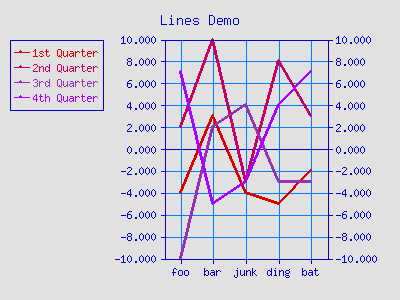
\includegraphics[scale=0.5]{d_lines2.png}
	\end{center}
	\caption{Lines chart}
	\label{fig:lines}
\end{figure}
\begin{verbatim}
use Chart::Lines;

$g = Chart::Lines->new();
$g->add_dataset ('foo', 'bar', 'junk', 'ding', 'bat');
$g->add_dataset ( -4,  3, -4, -5, -2);
$g->add_dataset (  2, 10, -3,  8,  3);
$g->add_dataset (-10,  2,  4, -3, -3);
$g->add_dataset (  7, -5, -3,  4,  7);

%hash = ('legend_labels' => ['1st Quarter', '2nd Quarter',
                             '3rd Quarter', '4th Quarter'],
         'y_axes' => 'both',
         'title' => 'Lines Demo',
         'grid_lines' => 'true',
         'legend' => 'left',
         'legend_example_size' => 20,
         'colors' => {'text' => 'blue',
                      'misc' => 'blue',
                      'background' => 'grey',
                      'grid_lines' => 'light_blue',
                      'dataset0' => [220,0,0],
                      'dataset1' => [200,0,100],
                      'dataset2' => [150,50,175],
                      'dataset3' => [170,0,255] },
         );

$g->set (%hash);

$g->png ("lines.png");
\end{verbatim}

\begin{Constructor} 
An instance of a lines chart object can be created with the constructor \textit{new()}:
\begin{quote}
\fett{\$obj = Chart::Lines->new();}\\
\fett{\$obj = Chart::Lines->new(\parameter{width}, \parameter{height});}
\end{quote}
If \textit{new()} has no arguments, 
the constructor returns an image with the size 300x400 pixels. If new has two arguments
\parameter{width} and \parameter{height}, it returns an image with the desired size.
\end{Constructor}

\Methods
\method{All universal valid methods, see page \pageref{methods} of \class{Chart::Base}.}\\[\parabstand]
%
\Attributes
All universal valid options, see page \pageref{options}. 
Special options for this type of chart are:\\
\begin{description}
\item['y\_axes'] Tells chart where to place the y-axis. 
                 Valid values are 'left', 'right' and 'both'. Defaults to 'left'.

\item['brush\_size'] Sets the width of the lines in pixels. Default is 6.

\item['xy\_plot'] Forces Chart to plot a x-y-graph, which means that the x-axis 
                  is also numeric if set to 'true'. 
                  Very useful for plots of mathematical functions. Defaults to 'false'.

\item['xlabels', 'xrange'] Allows the arbitrary positioning of the labels at the
                  x-axis. The option 'xy\_plot' must be defined to let this
                  options work. An example is
                  \begin{verbatim}
@labels = (['Jan', 'Feb','Mar'], 
           ['10','40','70']); 

$chart->set( xlabels => \@labels, 
             xrange => [0,100] 
           ); 
                   \end{verbatim}

\item['sort'] Sorts the data of a x-y-graph ascending if set to 'true'. 
              Should be set if the added data isn't sorted. Defaults to 'false'.   

\item['stepline'] The points are connected by a stepping function,
                  instead by a direct line if set to 'true'. 
                  Defaults to 'false'.   

\item['stepline\_mode'] Determine whether to start with the first point
                    (if set to 'begin') or end with the last point if set to 'end'.
                    Defaults to 'begin'.   
\end{description}



%
% linespoints.tex
%
\section{Chart::LinesPoints}
\name{Chart::LinesPoints}
\file{LinesPoints.pm}
\requires{Chart::Base, GD, Carp, FileHandle}
\begin{Description} 
\class{LinesPoints} is a subclass of \class{Chart::Base}.
The class \class{LinesPoints} creates a lines chart with points marking the 
individual koordinates of the data.
\end{Description}

\parindent 0pt{\large Example:}

\begin{figure}[h]
	\begin{center}
		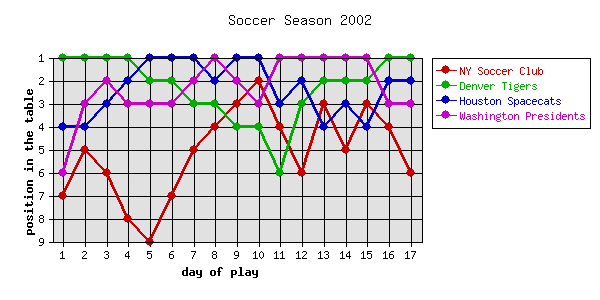
\includegraphics[scale=0.6]{d_linesp2.png}
	\end{center}
	\caption{Linespoints chart}
	\label{fig:d_linesp2}
\end{figure}
\begin{verbatim}
use Chart::LinesPoints;
use strict;

my (@data1, @data2, @data4, @data3, @labels, %hash, $g);

@labels = qw(1 2 3 4 5 6 7 8 9 10 11 12 13 14 15 16 17);
@data1 = qw (-7 -5 -6 -8 -9 -7 -5 -4 -3 -2 -4 -6 -3 -5 -3 -4 -6);
@data2 = qw (-1 -1 -1 -1 -2 -2 -3 -3 -4 -4 -6 -3 -2 -2 -2 -1 -1);
@data3 = qw (-4 -4 -3 -2 -1 -1 -1 -2 -1 -1 -3 -2 -4 -3 -4 -2 -2);
@data4 = qw (-6 -3 -2 -3 -3 -3 -2 -1 -2 -3 -1 -1 -1 -1 -1 -3 -3);

$g = Chart::LinesPoints->new(600,300);
$g->add_dataset(@labels);
$g->add_dataset(@data1);
$g->add_dataset(@data2);
$g->add_dataset(@data3);
$g->add_dataset(@data4);

%hash =(
          'integer_ticks_only' => 'true',
          'title' => 'Soccer Season 2002\n ',
          'legend_labels' => ['NY Soccer Club', 'Denver Tigers',
                              'Houston Spacecats', 'Washington Presidents'],
          'y_label' => 'position in the table',
          'x_label' => 'day of play',
          'grid_lines' => 'true',
          'f_y_tick' => \&formatter,
          );

$g->set ( %hash);
$g->png ("Grafiken/d_linesp2.png");

#just a trick, to let the y scale start at the biggest point:
#initiate with negative values, remove the minus sign!
sub formatter {
  my $label = shift;
  $label = substr($label, 1,2);
  return $label;
}

\end{verbatim}

\begin{Constructor} 
An instance of a linespoints chart object can be created with the constructor 
\textit{new()}:
\begin{quote}
\parindent 0pt
\fett{\$obj = Chart::LinesPoints->new();}\\
\fett{\$obj = Chart::LinesPoints->new(\parameter{width}, \parameter{height});}
\end{quote}

If \textit{new()} has no arguments, the constructor returns an image with the size 300x400 pixels.
If \textit{new()} has two arguments \parameter{width} and \parameter{height}, 
it returns an image with the desired size.
\end{Constructor}

\Methods
\method{All universal valid methods, see page \pageref{methods} of \class{Chart::Base}.} \\[\parabstand]
%
\Attributes
All universal valid options, see page \pageref{options}. 
Also available these special options:
\begin{description}
\item['y\_axes'] Tells chart where to place the y-axis. 
     Valid values are 'left', 'right' and 'both'. Defaults to 'left'.

\item['pt\_size'] Sets the radius of the points in pixels. Default is 18.

\item['brush\_size'] Sets the width of the lines in pixels. Default is 6.

\item['xy\_plot'] Forces Chart to plot a x-y-graph, 
                  which means that the x-axis is also numeric if set to 'true'. 
                  Very useful for plots of mathematical functions. Defaults to 'false'.

\item['sort'] Sorts the data of a x-y-graph ascending if set to 'true'. 
              Should be set if the added data isn't sorted. Defaults to 'false'.  
              
\item['stepline'] The points are connected by a stepping function,
                  instead by a direct line if set to 'true'. 
                  Defaults to 'false'.   

\item['stepline\_mode'] Determine whether to start with the first point
                    (if set to 'begin') or end with the last point if set to 'end'.
                    Defaults to 'begin'.   
\end{description}

\section{Chart::Mountain}
\herv{Name:} Chart::Mountain\\ \\
\herv{File:} Mountain.pm\\ \\
\herv{Requires:}Chart::Base, GD, Carp, FileHandle\\ \\
\herv{Description:} \fett{Mountain} is a \fett{subclass} of Chart::Base.\\
The class Mountain creates a mountain chart.\\
\\
\herv{Example:}
\begin{figure}[h]
	\begin{center}
		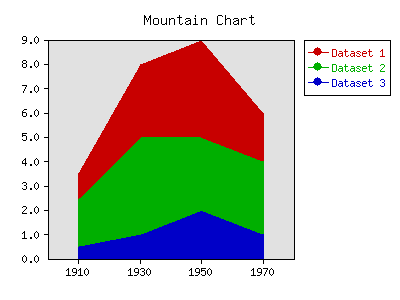
\includegraphics[scale =0.6]{mountain.png}
	\end{center}
	\caption{Mountain chart}
	\label{fig:mountain}
\end{figure}
\begin{verbatim}
use Chart::Mountain;

$g = Chart::Mountain->new();

@data = [ [1910, 1930, 1950, 1970],
          [1, 3, 4, 2],
          [2, 4, 3, 3],
          [0.5, 1, 2, 1]];

$g->set('title' => 'Mountain Chart',
        'grid_lines' => 'false',
        'precision' => 1);

$g->png("mountain.png", @data);

\end{verbatim}
\herv{Constructor:} An instance of a mountain chart object can be created with the constructor new():\\
\fett{\$obj = Chart::Mountain->new();}\\
\fett{\$obj = Chart::Mountain->new(\kursiv{width}, \kursiv{height});}\\
\\
If \fett{new} has no arguments, the constructor returns an image with the size 300x400 pixels. If new has two arguments \kursiv{width} and \kursiv{height}, it returns an image with the desired size. \\ 
\\ 
\herv{Methods:}All universally valid methods, see page \pageref{methods}: Chart::Base. \\
\\
\herv{Attributes/Options:} All universally valid options, see page \pageref{options}. Also available, these special options:
\begin{description}
\item['y\_axes'] Tells chart where to place the y-axis. Valid values are 'left', 'right' and 'both'. Defaults to 'left'.
\end{description}
\section{Chart::Pareto}
\herv{Name:} Chart::Pareto\\ \\
\herv{File:} Pareto.pm\\ \\
\herv{Requires:}Chart::Base, GD, Carp, FileHandle\\ \\
\herv{Description:} \fett{Pareto} is a \fett{subclass} of Chart::Base.\\
The class Pareto creates a pare-to chart. Pareto plots only one dataset and its labels.\\
\\
\herv{Example:}
\begin{figure}[h]
	\begin{center}
		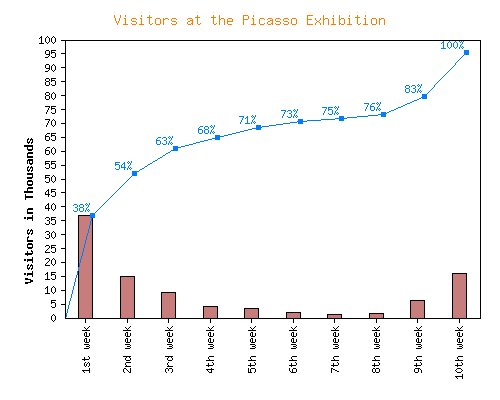
\includegraphics[scale=0.7]{d_pareto2.png}
	\end{center}
	\caption{Pare-to chart}
	\label{fig:pareto}
\end{figure}
\begin{verbatim}
use Chart::Pareto;

$g = Chart::Pareto->new(500,400);
$g->add_dataset ('1st week', '2nd week', '3rd week', '4th week', '5th week',
                 '6th week', '7th week', '8th week', '9th week', '10th week');
$g->add_dataset (37, 15, 9 , 4, 3.5,
                  2.1, 1.2, 1.5, 6.2, 16);

%hash =( 'colors' => { 'dataset0' => 'mauve',
                       'dataset1' => 'light_blue',
                       'title' => 'orange'},
         'title' => 'Visitors at the Picasso Exhibition',
         'integer_ticks_only' => 'true',
         'skip_int_ticks' => 5,
         'grey_background' => 'false',
         'max_val' => 100,
         'y_label' => 'Visitors in Thousands',
         'x_ticks' => 'vertical',
 	       'spaced_bars' => 'true',
         'legend' => 'none'
        );
	
$g->set (%hash); 
$g->png ("pareto.png");
\end{verbatim}
\herv{Constructor:} An instance of a pare-to chart object can be created with the constructor new():\\
\fett{\$obj = Chart::Pareto->new();}\\
\fett{\$obj = Chart::Pareto->new(\kursiv{width}, \kursiv{height});}\\
\\
If \fett{new} has no arguments, the constructor returns an image with the size 300x400 pixels. If new has two arguments \kursiv{width} and \kursiv{height}, it returns an image with the desired size. \\ 
\\ 
\herv{Methods:}All universally valid methods, see page \pageref{methods}: Chart::Base. \\
\\
\herv{Attributes/Options:} All universally valid options, see page \pageref{options}. Also available, these special options:
\begin{description}
\item['y\_axes'] Tells chart where to place the y-axis. Valid values are 'left', 'right' and 'both'. Defaults to 'left'.
\item['spaced\_bars']Leaves space between bars at each data point when set to 'true'.  This just makes it easier to read a bar chart.  Default is 'true'.
\item['sort']Sorts the data descending if set to 'true'. Defaults to 'false'.  
\end{description}
%
% pie.tex
%
\section{Chart::Pie}
\name{Chart::Pie}
\file{Pie.pm}
\requires{Chart::Base, GD, Carp, FileHandle}
\begin{Description} 
\class{Pie} is a subclass of class \class{Chart::Base}.
The class \class{Pie} creates a pie chart. The first added set are the labels. 
The second set are the values.
\end{Description}

\parindent 0pt{\large Example:}

\begin{figure}[h]
	\begin{center}
		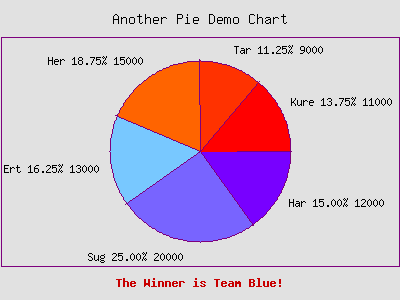
\includegraphics[scale = 0.6]{d_pie3.png}
	\end{center}
	\caption{Pie chart}
	\label{fig:pie}
\end{figure}
\begin{verbatim}
use Chart::Pie;

$g = Chart::Pie->new();

$g->add_dataset ('Har', 'Sug', 'Ert', 'Her', 'Tar', 'Kure');
$g->add_dataset (12000, 20000 , 13000, 15000, 9000, 11000  );

%opt = ( 'title' => 'Another Pie Demo Chart',
         'label_values' => 'both',
         'legend' => 'none',
         'text_space' => 10,
         'png_border' => 1,
         'graph_border' => 0,
         'colors' => { 'x_label' => 'red',
                       'misc' => 'plum',
                       'background' => 'grey',
                       'dataset0' => [120, 0, 255],
                       'dataset1' => [120, 100, 255],
                       'dataset2' => [120, 200, 255],
                       'dataset3' => [255, 100, 0],
                       'dataset4' => [255, 50, 0],
                       'dataset5' => [255, 0, 0],
                     },
         'x_label' => 'The Winner is Team Blue!',
        );

$g->set (%opt);

$g->png ("pie.png");
\end{verbatim}

\begin{Constructor} 
An instance of a pie chart object can be created with the constructor \textit{new()}:
\begin{quote}
\fett{\$obj = Chart::Pie->new();}\\
\fett{\$obj = Chart::Pie->new(\parameter{width}, \parameter{height});}
\end{quote}

If \textit{new()} has no arguments, 
the constructor returns an image with the size 300x400 pixels. 
If \textit{new()} has two arguments \parameter{width} and \parameter{height}, 
it returns an image within the desired size.
\end{Constructor}

\Methods
All universal valid methods, see page \pageref{methods} of class \class{Chart::Base}.\\[\parabstand]
%
\Attributes
All universal valid options, see page \pageref{options}. 
Also available, these special options:
\begin{description}
\item['label\_values'] 
          Tells the pie chart what labels to draw beside the pie. 
          Valid values are 'percent', 'value', 'both' and 'none'. Defaults to 'percent'.

\item['legend\_label\_values'] 
          Tells the pie chart what labels to draw in the legend. 
          Valid values are 'percent', 'value', 'both' and 'none'. Defaults to 'value'.
          
\item['legend\_lines']
          The labels drawn aside the pie are connected with a line to the segment.
          
\item['ring']
          The pie has a ring structure.          

\end{description}

%
% points.tex
%
\section{Chart::Points}
\name{Chart::Points}
\file{Points.pm}
\requires{Chart::Base, GD, Carp, FileHandle}
\begin{Description} 
\class{Points} is a subclass of class \class{Chart::Base}.\\
The class Points creates a point chart.
\end{Description}

\parindent 0pt{\large Example:}

\begin{figure}[h]
	\begin{center}
		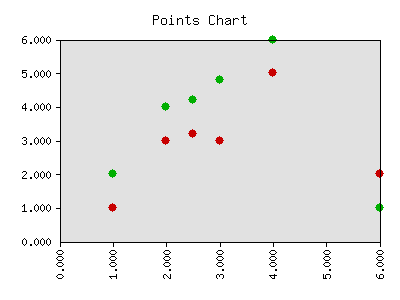
\includegraphics[scale=0.5]{points.png}
	\end{center}
	\caption{Points chart}
	\label{fig:points}
\end{figure}
\begin{verbatim}
use Chart::Points;

$g = Chart::Points->new();
$g->add_dataset (1, 4,   3, 6, 2, 2.5);  # x-coordinates
$g->add_dataset (1, 5,   3, 2, 3, 3.2);  # y-coordinates dataset 1
$g->add_dataset (2, 6, 4.8, 1, 4, 4.2);  # y-coordinates dataset 2

@hash = ('title' => 'Points Chart',
         'xy_plot' => 'true',
         'x_ticks' => 'vertical',
         'legend' => 'none',
         'sort' => 'true',
         'precision' => 3,
         'include_zero' => 'true',
	 );

$g->set (@hash);

$g->png ("Grafiken/points.png");
\end{verbatim}

\begin{Constructor} 
An instance of a points chart object can be created with the constructor \textit{new()}:
\begin{quote}
\fett{\$obj = Chart::Points->new();}\\
\fett{\$obj = Chart::Points->new(\parameter{width}, \parameter{height});}
\end{quote}

If \textit{new()} has no arguments, 
the constructor returns an image with the size 300x400 pixels. If new has two arguments 
\parameter{width} and \parameter{height}, 
it returns an image with the desired size.
\end{Constructor}

\Methods
All universal valid methods, see page \pageref{methods} of class \class{Chart::Base}. \\[\parabstand]
%
\Attributes
All universal valid options, see page \pageref{options}. 
Also available these special options:
\begin{description}
\item['y\_axes'] Tells chart where to place the y-axis. 
                 Valid values are 'left', 'right' and 'both'. Defaults to 'left'.
                 
\item['pt\_size'] Sets the radius of the points in pixels. Default is 18.

\item['sort'] Sorts the data of a x-y-graph ascending if set to 'true'. 
              Should be set if the added data isn't sorted. Defaults to 'false'.
              
\item['xy\_plot'] Forces Chart to plot a x-y-graph, 
                  which means that the x-axis is also numeric if set to 'true'. 
                   Very useful for plots of mathematical functions. Defaults to 'false'.

\item['xlabels', 'xrange'] Allows the arbitrary positioning of the labels at the
                  x-axis. The option 'xy\_plot' must be defined to let this
                  options work. An example is
                  \begin{verbatim}
@labels = (['Jan', 'Feb','Mar'], 
           ['10','40','70']); 

$chart->set( xlabels => \@labels, 
             xrange => [0,100] 
           ); 
                   \end{verbatim}

\end{description}

%
% split.tex
%
\section{Chart::Split}
\name{Chart::Split}
\file{Split.pm}
\requires{Chart::Base, GD, Carp, FileHandle}
\begin{Description} 
\class{Split} is a subclass of class \class{Chart::Base}.\\
The class \class{Split} creates a lines chart. 
Split makes always an xy-plot, which means that both axes are numeric. 
The x-axis will be split in several parts of a same interval (option 'interval' has to be set!).
These intervals will be drawn one upon the other. 
The top interval starts at the start point, 
which has to be set by the programmer (option 'start'). \\
The first passed dataset are the x coordinates. 
The following added sets are the y coordinates of the sets.\\
Split draws only positive x-coordinates.\\
The y-axis is a numbering of the intervals.\\
The Split module is useful if you have a lot of data points to plot. An example is to plot
weather or seismic data.
\end{Description}

\parindent 0pt{\large Example:} 

\begin{figure}[h]
	\begin{center}
		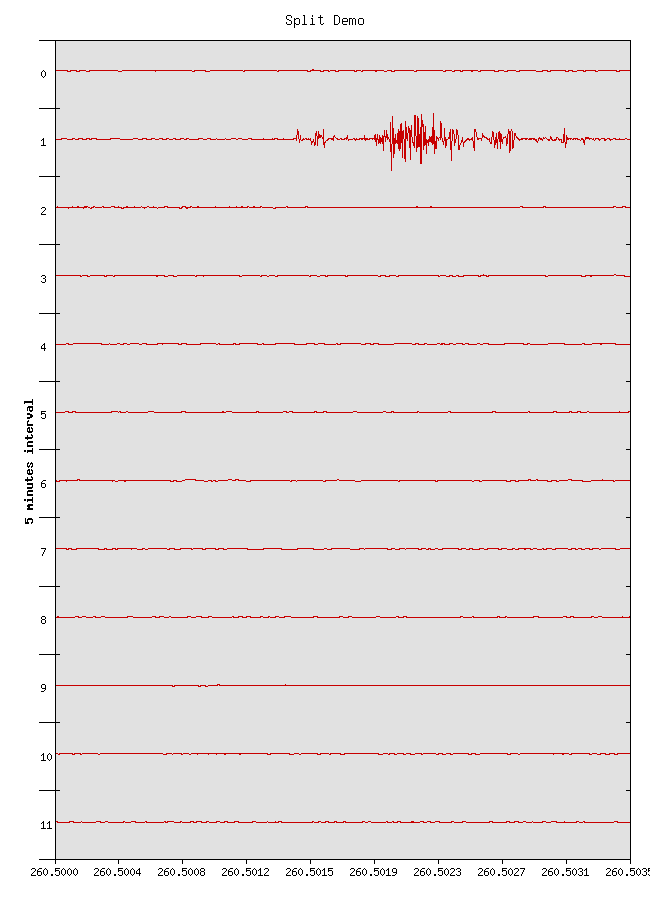
\includegraphics[width = 10cm, height =10cm]{stunde.png}
	\end{center}
	\caption{Split chart}
	\label{fig:split}
\end{figure}
\begin{verbatim}
use Chart::Split;

$g = Chart::Split->new(650 ,900);

#get the data that are in a file and push them in arrays
open( FILE , "data.dat") or die 'Can't open the data file!\n';
while (defined ($line = <FILE>) ) {
  ($x, $y,) = unpack("a11 x1 a8" , $line);
   push (@y, $y);
   push (@x, $x);
}
close (FILE);

#add the data
$g->add_dataset(@x);
$g->add_dataset(@y);

#set the options
$g->set('xy_plot' => 'true');
$g->set('legend' => 'none');
$g->set('title' => 'Split Demo');
$g->set('interval' => 1/288);
$g->set('interval_ticks' => 10);
$g->set('start' => 260.5);
$g->set('brush_size' => 1);
$g->set('precision' => 4);
$g->set('y_label' => '5 minutes interval');

#give me a nice picture
$g->png("split.png");
\end{verbatim}

\begin{Constructor} 
An instance of a split chart object can be created with the constructor \textit{new()}:
\begin{quote}
\fett{\$obj = Chart::Split->new();}\\
\fett{\$obj = Chart::Split->new(\parameter{width}, \parameter{height});}
\end{quote}

If \textit{new()} has no arguments, 
the constructor returns an image with the size 300x400 pixels. If new has two arguments 
\parameter{width} and \parameter{height}, it returns an image with the desired size.
\end{Constructor}

\Methods
All universal valid methods, see page \pageref{methods} of class
\class{Chart::Base}.\\[\parabstand]
%
\Attributes
All universal valid options, see page \pageref{options}. 
Also available, these special options:
\begin{description}
\item['start'] \emph{Required} value for a split chart. \\
               If the x coordinate of the first data point is zero, 
               you should set start to zero. 
               Sets the start value of the first interval. Defaults to undef.
               
\item['interval'] \emph{Required} value of a split chart.\\
                Sets the interval of one line to plot. Defaults to undef.
                
\item['interval\_ticks'] Sets the number of ticks for the x-axis. Defaults to 5.

\item['scale'] Every y-value of a split chart will be multiplied by that value, 
               but the scale won't be changed. This means you may overdraw certain rows! 
               Only useful if you want to give prominence to the maximal amplitudes of the data.
               Defaults to 1.
               
\item['sort'] Sorts the data ascending if set to 'true'. 
              Should be set if the added data isn't sorted. Defaults to 'false'.  
              
\item['y\_axes'] Tells chart where to place the y-axis. 
                 Valid values are 'left', 'right' and 'both'. Defaults to 'left'.
\end{description}

%
% stacked.tex
%
\section{Chart::StackedBars}
\name{Chart::StackedBars}
\file{StackedBars.pm}
\requires{Chart::Base, GD, Carp, FileHandle}
\begin{Description} 
\class{StackedBars} is a \fett{subclass} of class \class{Chart::Base}.
The class StackedBars creates a chart with stacked bars.
\end{Description}

\parindent 0pt{\large Example:}

\begin{figure}[h]
	\begin{center}
		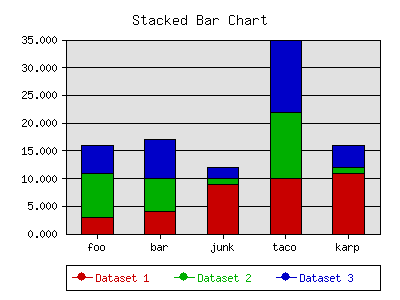
\includegraphics[scale=0.6]{stackedbars.png}
	\end{center}
	\caption{Chart with stacked bars}
	\label{fig:stackedbars}
\end{figure}
\begin{verbatim}
use Chart::StackedBars;

$g = Chart::StackedBars->new;

$g->add_dataset ('foo', 'bar', 'junk', 'taco', 'karp');
$g->add_dataset (3, 4, 9, 10, 11);
$g->add_dataset (8, 6, 1, 12, 1);
$g->add_dataset (5, 7, 2, 13, 4);

$g->set ('title' => 'Stacked Bar Chart');
$g->set('y_grid_lines' => 'true');
$g->set('legend' => 'bottom');

$g->png ("Grafiken/stackedbars.png");
\end{verbatim}

\begin{Constructor} An instance of a stacked bars object can be created with the constructor
\textit{new()}:
\begin{quote}
\fett{\$obj = Chart::StackedBars->new();}\\
\fett{\$obj = Chart::StackedBars->new(\parameter{width}, \parameter{height});}
\end{quote}
If \textit{new()} has no arguments, 
the constructor returns an image with the size 300x400 pixels. 
If \textit{new()} has two arguments \parameter{width} and \parameter{height},
it returns an image with the desired size.
\end{Constructor}

\Methods
All universal valid methods, see page \pageref{methods}
of class \class{Chart::Base}.\\[\parabstand]
%
\Attributes
All universal valid options, see page \pageref{options}. Also available, these special options:
\begin{description}
\item['y\_axes'] Tells chart where to place the y-axis. 
                 Valid values are 'left', 'right' and 'both'. Defaults to 'left'.
\item['spaced\_bars'] Leaves space between the groups of bars at each data point 
                      when set to 'true'.  
                      This just makes it easier to read a bar chart.  Default is 'true'.
\end{description}

\listoffigures
\printindex

\end{document}
